\chapter{ Экспериментальный раздел}
Результаты работы алгоритмов представлены в таблицах \ref{table:even} и \ref{table:noneven}(для четных и нечетных размерностей матриц). Полученные данные представлены в виде диаграмм изображенных на рисунках \ref{figure:evenImg} и \ref{figure:nonEvenImg}

1 -- Классический алгоритм Винограда(на графиках представлен черным цветом)

2 -- Оптимизированный алгоритм Винограда(на графиках представлен красным цветом)

3 -- Последовательное перемножение матриц(на графиках представлен синим цветом)

\begin{table}
	\caption{Таблица для сравнения результатов работы алгоритма для четной размерности в микросекундах.}\label{table:even}
	\begin{center}
		\begin{tabular}{cccc}
            \textbf{Размер} & \textbf{1} & \textbf{2} & \textbf{3}\\
            \textbf{100 X 100} & 20.077 & 20.859 & 25.865 \\
            \textbf{200 X 200} & 258.613 & 154.072 & 201.215 \\
            \textbf{300 X 300} & 536.736 & 516.737 & 687.302 \\
            \textbf{400 X 400} & 1277.363 & 1229.492 & 1657.234 \\
            \textbf{500 X 500} & 2508.538 & 2408.629 & 3294.885 \\
            \textbf{600 X 600} & 4878.377 & 4685.910 & 6107.689 \\
            \textbf{700 X 700} & 7778.614 & 7495.057 & 9871.546 \\
            \textbf{800 X 800} & 11597.817 & 11170.562 & 14822.127 \\
            \textbf{900 X 900} & 16712.889 & 16070.812 & 21545.400 \\
            \textbf{1000 X 1000} & 23102.137 & 22225.149 & 29986.602 \\
		\end{tabular}
	\end{center}
\end{table}

\begin{table}
		\caption{Таблица для сравнения результатов работы алгоритма для нечетной размерности в микросекундах.}\label{table:noneven}
	\begin{center}
		\begin{tabular}{cccc}
            \textbf{Размер} & \textbf{1} & \textbf{2} & \textbf{3}\\
            \textbf{101 X 101} & 20.809 & 21.282 & 26.734 \\
            \textbf{201 X 201} & 161.322 & 156.745 & 204.425 \\
            \textbf{301 X 301} & 541.239 & 525.954 & 692.841 \\
            \textbf{401 X 401} & 1284.754 & 1236.969 & 1685.261 \\
            \textbf{501 X 501} & 2528.653 & 2422.614 & 3316.100 \\
            \textbf{601 X 601} & 4918.674 & 4727.957 & 6148.991 \\
            \textbf{701 X 701} & 7833.712 & 7528.168 & 9911.066 \\
            \textbf{801 X 801} & 11725.979 & 11282.570 & 15007.543 \\
            \textbf{901 X 901} & 16744.922 & 16120.746 & 21658.227 \\
            \textbf{1001 X 1001} & 23189.963 & 22264.232 & 30098.645 \\
		\end{tabular}
	\end{center}
\end{table}

\begin{figure}[ht!]
	\centering{ 
		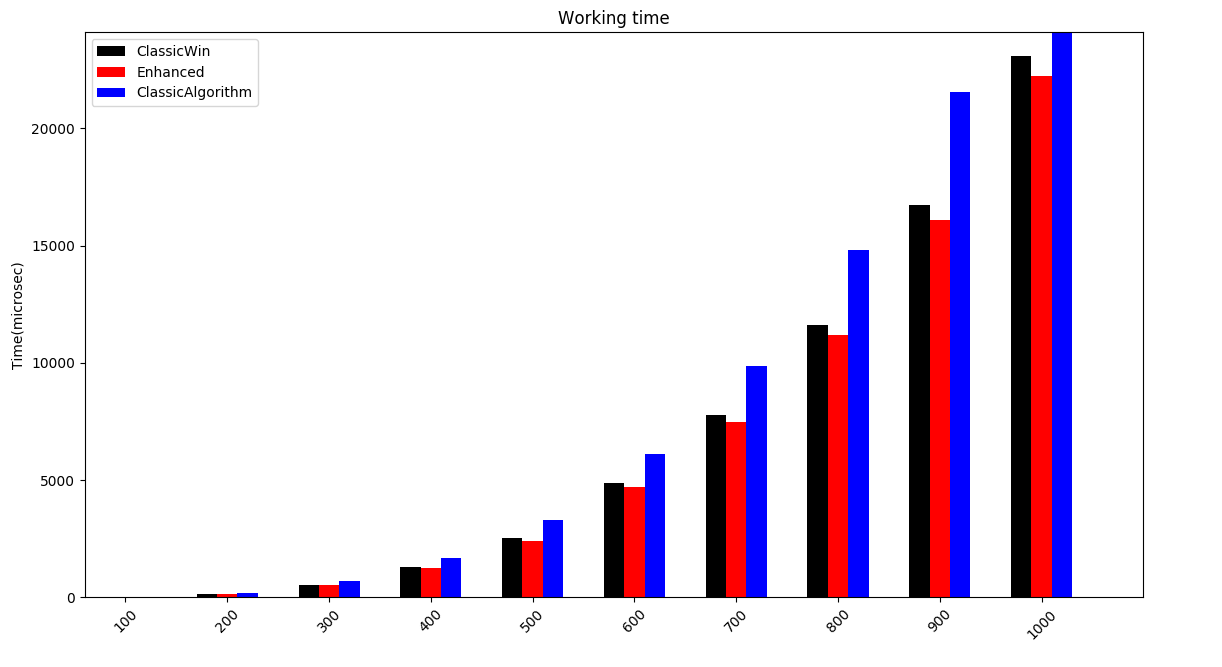
\includegraphics[width=1.1\textwidth]{img/evenAdd.png}
        \caption{График для квадратных матриц четной размерности}\label{figure:evenImg}}
\end{figure}

\begin{figure}[ht!]
	\centering{ 
		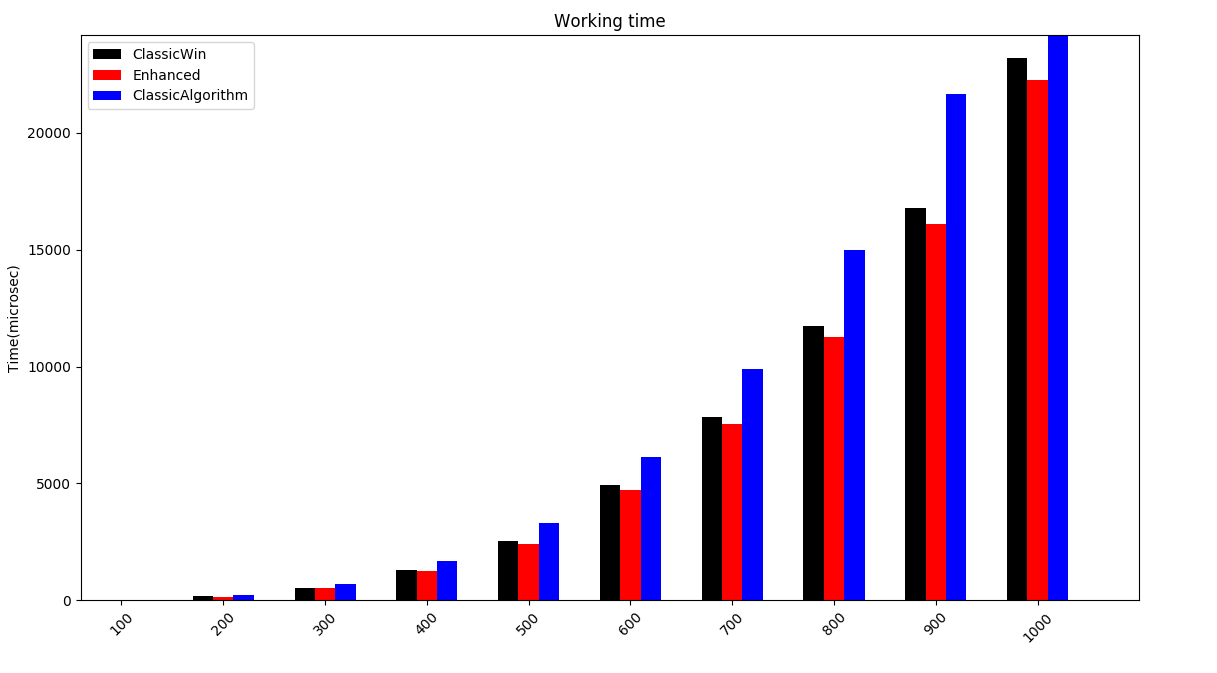
\includegraphics[width=1.1\textwidth]{img/nonEvenAdd.png}
        \caption{График для квадратных матриц нечетных размерностей}\label{figure:nonEvenImg}}
\end{figure}

По полученным данным можно сделать вывод, что стандартный алгоритм перемножения матриц работает медленнее, чем классический алгоритм Винограда и улучшенный алгоритм Винограда. Улучшенный алгоритм работает быстрее по времени, чем классический. Если обратиться к рассчитанным трудоемкостям алгоритмов, можно заметить, что стандартный алгоритм менее трудоемкий, чем два других, но время, затрачиваемое на рассчет матрицы стандартным методом все равно очень большое. Так как это зависит от модели вычислений, где умножение и обращения к индексам и сложение были взяты за 1, можно сказать, что следует учитывать некоторые ньюансы при выборе весов операций, чтобы вычесленная трудоемкость была более точной.
